\documentclass[sans,mathserif]{beamer}
%handout,notes=show

%\usepackage{pgfpages}
%\pgfpagesuselayout{8 on 1}[a4paper,border shrink=5mm]

\usetheme{default}
\usepackage{fp}
\usepackage[thicklines]{cancel}
\usepackage{tikz}
\usepackage{multirow}
\usepackage{amsmath}
\usepackage{ifthen}
\usepackage{animate}
\usepackage{setspace}
\usepackage{forloop}
\usepackage{tikz}

%\usepackage{concmath}
%\usepackage{pxfonts}
%\usepackage{eulervm}
%\usepackage{mathpazo}
%\renewcommand\mathfamilydefault{\rmdefault}

%\usefonttheme{professionalfonts}
%\setmathfont{}
%\setsansfont{Palatino}
\usetikzlibrary{arrows,backgrounds,positioning,fit,chains,shapes,calc}

%\usepackage{handoutWithNotes}
%\pgfpagesuselayout{4 on 1 with notes}[a4paper,border shrink=5mm]

\setbeamertemplate{navigation symbols}{}

\title{Hashdist -- A tool for building and managing your scientific software distribution(s)}
\author{Chris Kees (US Army ERDC) and the HashDist Developers}
\institute{Coastal and  Hydraulics Laboratory \\ U.S. Army ERDC}
\date{Sage Days 58, June 16-20, 2014}

\newcommand{\V}{\vskip1em}

\setbeamersize{sidebar width left=0cm, sidebar width right=0cm}
\setbeamersize{text margin left=.8cm, text margin right=.8cm}

\defbeamertemplate{note page}{infolines}
{%
  \vskip3em
%  \setstretch{1.8}
  \Large
  \rmfamily
  \insertnote
}
\setbeamertemplate{note page}[infolines]

\renewcommand{\CancelColor}{\color{red}}

\begin{document}


\begin{frame}
  \titlepage

  \begin{center} {\tt http://github.com/hashdist}
  \end{center}
~
\end{frame}

\begin{frame}
  \frametitle{Acknowledgements}
\begin{itemize}
\item Dag Sverre Seljebotn, Ond\v{r}ej \v{C}ert\'{i}k, Aron Ahmadia, Robert Maynord, Jimmy Tang, Lane Wittgen,...
\item Dag Sverre's work for Simula Innovation was funded by a grant from the International Research Office, US Army Engineer Research and Development Center (BAA contract W911NF-12-1-0604)
\item Ond\v{r}ej's work for UT was funded by the US Army Engineer Research and Development Center (BAA Contract BAA12-4941) 
\item Part of Aron's work was supported by the CHL Research Participation Program administered by Oak Ridge Institute for Science and Education
\end{itemize}
\end{frame}

\begin{frame}
\frametitle{What's the problem?}
\begin{itemize}
\item<+-> I wrote some math software and I want YOU to use it.
\item<+-> Problem: My software needs libfoo, which you don't have.
\item<+-> Problem: My software needs libfoo, which you  DO have in a really weird location.
\item<+-> Problem: I built my software on an old linux  machine,  you need  it on OS X.
\item<+-> Problem: You need to run my software on an HPC machine.
\item<+-> Problem: You don't have  root access to your machine.
\item<+-> Solution: I need to add my software to a distribution that can handle all these cases.
\end{itemize}
\end{frame}

\begin{frame}
  \frametitle{Rest of the world in 2013, 2014?,...}
  \begin{itemize}
    \item<+-> Debian/RedHat distributions (linux only)
    \item<+-> App store (mac only)
    \item<+-> Web apps (still needs good distribution)
    \item<+-> Matlab environment (a kind of distribution)
    \item<+-> Modules on HPC machines.
  \end{itemize}
\end{frame}

\begin{frame}
\frametitle{Background}
\begin{itemize}
\item Proteus toolkit for PDE's was building its own stack with custom scripts, makefiles, and config files
\item FENICS  toolkit  for PDE's had its own system (Dorsal)
\item Various other DoD groups had their own Python distributions
\item Could possibly have added  to sage or enthough distributions but would require many new packages
\end{itemize}
\end{frame}

\begin{frame}
\frametitle{Requirments for new system}
\begin{itemize}
\item Must support mixing source and ``host'' packages (e.g. vendor MPI)
\item Must support version control and reproducibility across  users
\item Must support many kinds of packages (Python, C++, Fortran,...)
\item Must support needs of developers (building from git repos, trying new packages,...)
\end{itemize}
\end{frame}

\begin{frame}
  \frametitle{Scientific code}
  \begin{itemize}
  \item<+-> Dependencies are bad: Hard to build, move between clusters
  \item<+-> Dependencies are good: Can build on works of others
  \item<+-> Often happens: ``Large frameworks'' bundling things together
    \begin{itemize}
    \item<+-> PETSc and Trilinos for solving PDEs
    \item<+-> As soon as you want to push boundaries there's a lot of dirty work ahead
    \end{itemize}
  \end{itemize}
\end{frame}

\begin{frame}[fragile]
  \frametitle{What makes scientific codes so special?}

  \begin{itemize}
    \item<+-> No root access
    \item<+-> Sometimes you {\bf need} the very latest version
    \item<+-> Fortran/C++ instead of C/Java/.NET
    \item<+-> Intersection of ``need speed'' and ``do not pay dedicated application sysadmins''
  \end{itemize}
\end{frame}

\begin{frame}[fragile]
  \frametitle{Combinatorial explosion}

\uncover<+->{
\small {\tt

/cluster/software/VERSIONS/hdf5-1.6.1/lib/libhdf5.so \\
/cluster/software/VERSIONS/hdf5-1.6.1\_intel/lib/libhdf5.so \\
/cluster/software/VERSIONS/hdf5-1.6.1\_pgi/lib/libhdf5.so \\
/cluster/software/VERSIONS/hdf5-1.8.9/lib/libhdf5.so \\
/cluster/software/VERSIONS/hdf5-1.8.9\_intel/lib/libhdf5.so \\
/cluster/software/VERSIONS/hdf5-1.8.9\_pgi/lib/libhdf5.so \\
}}

~

\uncover<+->{
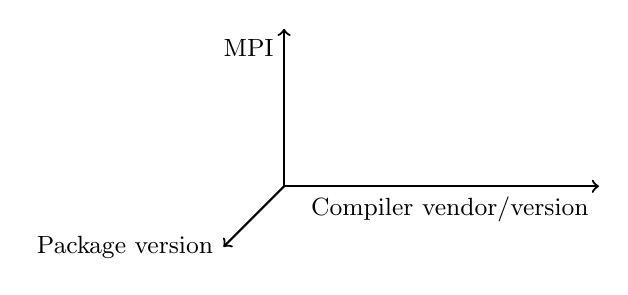
\begin{tikzpicture}[scale=2]
    \draw[thick,->,black] (0,0,0) -- (2,0,0) node[anchor=north east]{\small Compiler vendor/version};
    \draw[thick,->] (0,0,0) -- (0,1,0) node[anchor=north east]{\small MPI};
    \draw[thick,->] (0,0,0) -- (0,0,1) node[anchor=east]{\small Package version};
\end{tikzpicture}

~

$\times$ LAPACK $\times$ FFT library $\times$ IDL/Python version...
}

\end{frame}



\begin{frame}
  \frametitle{Established options elsewhere}

  \begin{itemize}
  \item<+-> Debian/Ubuntu/RedHat/Gentoo
    \begin{itemize}
    \item<+-> Need root
    \item<+-> Deals poorly with combinatorial explosion
    \end{itemize}
  \item<+-> MacPorts, Fink
    \begin{itemize}
    \item<+-> Mac only
    \item<+-> Deals ``not good enough'' with combinatorial explosion
    \end{itemize}
  \item<+-> HPC environment modules
    \begin{itemize}
    \item<+-> The sysadmins hate them
    \item<+-> The users need newer/their own libraries
    \end{itemize}
  \end{itemize}

\end{frame}

\begin{frame}
  \frametitle{Current solutions}
  \begin{itemize}
  \item<+-> Build yourself from source
    \begin{itemize}
    \item<+-> {\tt ./configure -\,{}-prefix=\$HOME/local; make; make install}
    \item<+-> {\tt export LD\_LIBRARY\_PATH=\textasciitilde{}sigurdkn/local/lib}
    \item<+-> Fragile, duplication of work...
    \end{itemize}
  \item<+-> Aha! Make a script to build from source...
    \begin{itemize}
    \item Simula: dorsal
    \item 5 different within DoD (incl. python-hpcmp)
    \item Sage
    \item Lots of others (``everybody'' does it)
    \end{itemize}
  \item<+-> Easy to do oneself $\Rightarrow$ difficult for one to get
    momentum
  \item<+-> The details are different for everybody
  \end{itemize}

\end{frame}


\begin{frame}
  \frametitle{Curation}
  
  \begin{itemize}
  \item<+-> Debian, RedHat, cluster sysadmins, dorsal is all about curated software stacks
  \item<+-> Perhaps you want 60\% curated, 20\% bleeding edge or manually tweaked, 20\% your own code...
  \item<+-> The community using and supporting a distribution is as  important as  most of the other details. 
  \end{itemize}
\end{frame}

\begin{frame}
  \begin{center}
    {\Large HashDist Theory}
  \end{center}
\end{frame}

\begin{frame}
\frametitle{Stateful vs. Functional}
\begin{itemize}
\item<+-> Our software environment is usually defined by the STATE of the file system
\item<+-> If I change the source or options for libfoo, then I rebuild
  it in /usr/lib/libfoo.so.
\item<+-> Stateful systems are fine when you control everything (a
  linux distribution, sage distribution)
\item<+-> An alternative view is to think of the build stage as a
  mapping from the input  domain (input space $=$ dependency states  $\oplus$ source code states $\oplus$ option states) to a range
  containing binary ``artifacts'' (output space of ``coordinates'' of unique libfoo.a's).
\item<+-> Main idea: create build artifact coordinates by hashing the input state and store  the build artifacts in a ``database'' keyed  on those hashes.
\item<+-> Using the hash idea we can treat package building in a functional manner rather than a stateful manner (idea comes from Eelco Doltstra/Nix)
\end{itemize}
\end{frame}

\begin{frame}
  \frametitle{Cryptographic/secure hashing}

  \begin{itemize}
  \item<+-> Large key size (160, 256, or 512 bits)
    \begin{itemize}
    \item NIST standards: SHA-1, SHA-2 (224, 256, 384, 512 bits), SHA-3
    \end{itemize}
  \item<+-> Mathematical research topic to make $h$ such that no
    information about input is revealed
  \end{itemize}

~

\uncover<+->{
\small
\only<3>{$h$({\tt 'The dark fox'}) = $h$({\tt 546865206461726b20666f78} hex) \\
\quad  = {\tt b6589fc6ab0dc82cf12099d1c2d40ab994e8410c} hex}
\only<4>{$h$({\tt 'The dark fog'}) = $h$({\tt 546865206461726b20666f67} hex) \\
\quad  = {\tt da4b9237bacccdf19c0760cab7aec4a8359010b0} hex}%
}


\end{frame}

\begin{frame}
  \frametitle{Example: git}
~

\only<1>{

\tt
\$ (cd code/hashdist/.git/objects; find)
./59/5a2f8e3890d0ece24514f3e32ae874f1f03ac2 \\
./2f/780151688e1f122a5b9072d42009c80c36140c \\
./2f/4b2eef40b51bc2d46027d1864653b37dd05f8f \\
./2f/237d74e3f81f498212629ac0b96bedac4b0b36 \\
./2f/dff799c54fed6fe96a91e1d5f1593996228ebc \\
./2f/27bd4efa5f8521fb98eb82181a67aae97b7f1a \\
./2f/3fedf882f1b28905199961356f4e00281ddf76 \\
}
\only<2->{
  \begin{center}
    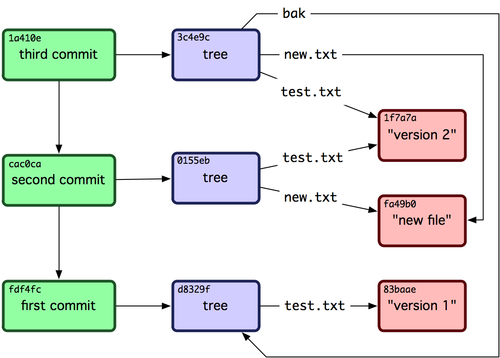
\includegraphics[width=.8\textwidth]{githashes.png}
  \end{center}
}
\end{frame}

\begin{frame}
  \begin{center}
    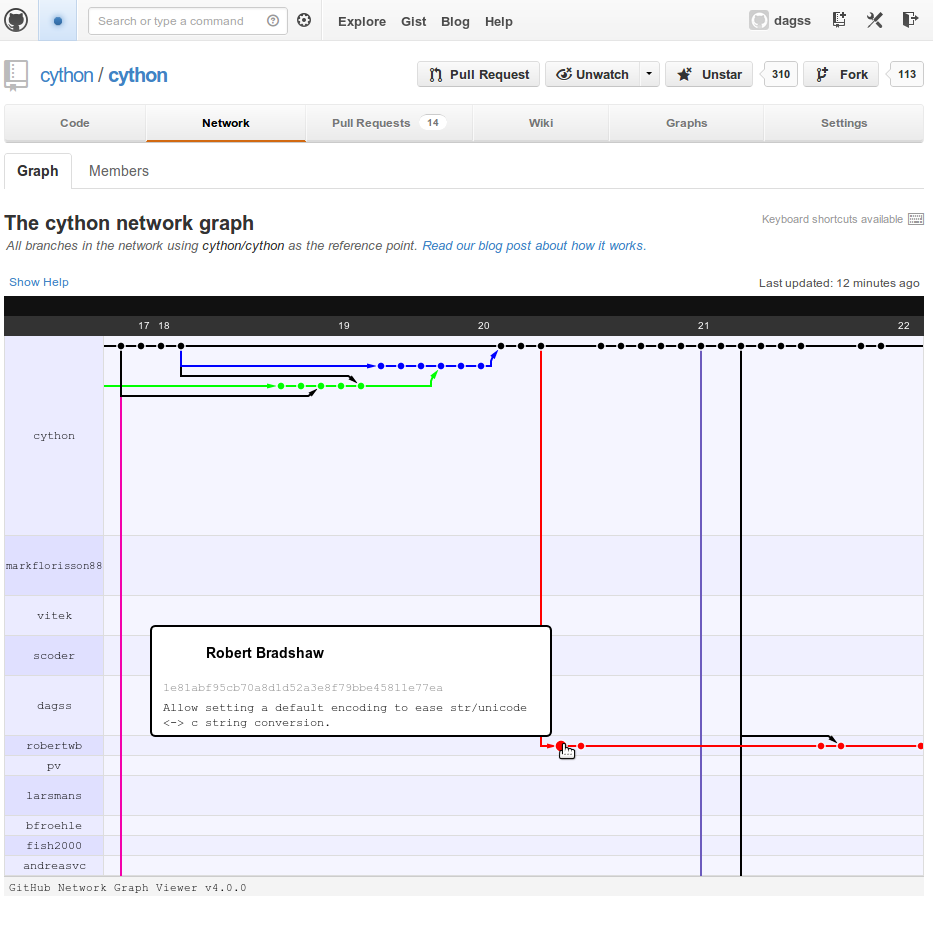
\includegraphics[width=.9\textwidth]{github-screendump.png}
  \end{center}
\end{frame}

\begin{frame}
  \begin{center}
    {\LARGE Hashdist}
  \end{center}
\end{frame}

\begin{frame}[fragile]
  \frametitle{Hash-based installation}

  \begin{itemize}
  \item<+-> Linux laptop:
{\small
\begin{semiverbatim}
/usr/lib/libhdf5.so
\end{semiverbatim}
}
  \item<+-> HPC environment modules:
{\small
\begin{semiverbatim}
/cluster/software/VERSIONS/hdf5-1.6.1/lib/libhdf5.so
/cluster/software/VERSIONS/hdf5-1.6.1_intel/lib/libhdf5.so
/cluster/software/VERSIONS/hdf5-1.6.1_pgi/lib/libhdf5.so
/cluster/software/VERSIONS/hdf5-1.8.9/lib/libhdf5.so
/cluster/software/VERSIONS/hdf5-1.8.9_intel/lib/libhdf5.so
/cluster/software/VERSIONS/hdf5-1.8.9_pgi/lib/libhdf5.so
\end{semiverbatim}

  \begin{itemize}
  \item<+-> Even {\tt
      h5py-hdf5\_1.8.9\_pgi-python2.7-numpy1.6.3\_abel\_debug}
    incomplete
  \item<+-> Abel is new and small; US Army clusters have 20-30 versions of every package.
  \end{itemize}
}
    \item<+-> Hashdist:
{\small 
\begin{semiverbatim}
~/.hashdist/bld/hdf5/pe7l56vsgg43
~/.hashdist/bld/hdf5/tkiwsppxzc3r
\end{semiverbatim}
}
{\footnotesize (really {\tt hdf5/tkiwsppxzc3ro3q7pyjjxq45jgh3wwcd})}
  \end{itemize}
\end{frame}

\begin{frame}[fragile]
  \frametitle{Step 1: Hash the build}
\uncover<+->{{\bf Internal protocol!}}
{\footnotesize
\begin{semiverbatim}
\{
  "build" : \{
    "commands" : [
      \{
        "cmd" : [
          "$BASH", 
          "\_hashdist/build.sh"
        ]
      \}, 
    ], 
    "import" : [
      \{
        "id" : "zlib/3vq2jgzdjakdhpzvpvtrbzbcrtg6etrh", 
        "ref" : "ZLIB"
      \}
    ]
  \}, 
  "name" : "hdf5", 
  "sources" : [
    \{
      "key" : "tar.bz2:l2q3vax4o42q5zriw6k243w6ax7ov4og", 
      "target" : "."
    \}
  ]
\}
\end{semiverbatim}
}

~

\uncover<+->{Hash to create key $\rightarrow$
\only<2>{{\tt \footnotesize hdf5/u4vsabroylchvmwoxf5mdpxidd4lnrwl}}%
\only<3->{{\color{red} \tt \footnotesize hdf5/fjczhadqtyx6jlbnvzlthrzsex7wz7xb}}
}

\end{frame}

\begin{frame}[fragile]
  \frametitle{Step 2: Every build installs to separate location}
Same as with the ``module load`` system:

\begin{semiverbatim}
\$ echo bld/*/* bld/adh/hwz2wmrcnbj7 bld/adh/lvpjelejrldo
bld/bzip2/zuo2tlurm7ez bld/cython/bidpqe4yx6gl bld/cython/pbdoyxvljz6u
bld/cython/xoju62amg7pm bld/daetk/dpoolktbk3si
bld/docutils/ckp3lhso6vek bld/docutils/uv2667zawv7v
bld/docutils/yekwczohjna7

\$ ls bld/zmq/x7ogmtwtkola/lib
pkgconfig  libzmq.a  libzmq.so  libzmq.so.3  libzmq.so.3.0.0

\end{semiverbatim}
\end{frame}

\begin{frame}[fragile]
  \frametitle{Step 2: Every build installs to separate location}
Unlike ``module load`` we don't need LD\_LIBRARY\_PATH:
\begin{semiverbatim}
\$ ldd bld/hdf5/tkiwsppxzc3r/lib/libhdf5.so
	linux-vdso.so.1 =>  (0x00007fffe21fe000)
	libpthread.so.0 => /lib/x86_64-linux-gnu/libpthread.so.0 (0x00007f9d0d2a4000)
	libz.so.1 => /home/cekees/.hashdist/bld/zlib/3vq2jgzdjakd/lib/libz.so.1 (0x00007f9d0d08a000)
	libdl.so.2 => /lib/x86_64-linux-gnu/libdl.so.2 (0x00007f9d0ce86000)
	libm.so.6 => /lib/x86_64-linux-gnu/libm.so.6 (0x00007f9d0cb80000)
	libmpich.so.10 => /home/cekees/.hashdist/bld/mpich/4ztabf2u23u2/lib/libmpich.so.10 (0x00007f9d0c71a000)
	libc.so.6 => /lib/x86_64-linux-gnu/libc.so.6 (0x00007f9d0c354000)
	/lib64/ld-linux-x86-64.so.2 (0x00007f9d0d9dc000)
	libmpl.so.1 => /home/cekees/.hashdist/bld/mpich/4ztabf2u23u2/lib/libmpl.so.1 (0x00007f9d0c14f000)
	librt.so.1 => /lib/x86_64-linux-gnu/librt.so.1 (0x00007f9d0bf46000)
	libgcc_s.so.1 => /lib/x86_64-linux-gnu/libgcc_s.so.1 (0x00007f9d0bd30000)
\end{semiverbatim}
\end{frame}


\begin{frame}[fragile]
\frametitle{Step 3: Make a profile with links}
\begin{semiverbatim}
\$ ls -la bld/profile/ycz6e4bztfgd/bin
bunzip2 -> ../../../bzip2/zuo2tlurm7ez/bin/bunzip2
bzcat -> ../../../bzip2/zuo2tlurm7ez/bin/bzcat
bzcmp -> ../../../bzip2/zuo2tlurm7ez/bin/bzcmp
...
\end{semiverbatim}
\end{frame}


\begin{frame}[fragile]
\frametitle{Branchable software stack}

\begin{itemize}
\item<+->
\begin{semiverbatim}
\textasciitilde{}/mystack \$ ls
default.yml sources.yml build.yml abel-cluster.yml
\end{semiverbatim}

\item<+->
\begin{semiverbatim}
\textasciitilde{}/mystack \$ hit build # takes some time
\textasciitilde{}/mystack \$ ~/local/bin/python --version
Python 2.7.2
\end{semiverbatim}
\item<+->
\begin{semiverbatim}
\textasciitilde{}/mystack \$ hit build # instant
\end{semiverbatim}

\item<+->
\begin{semiverbatim}
\textasciitilde{}/mystack \$ git fetch from-someone-else
\textasciitilde{}/mystack \$ git checkout someone-elses-branch
\textasciitilde{}/mystack \$ hit build # pause for extra builds
\textasciitilde{}/mystack \$ ~/local/bin/python --version
Python 2.7.3
\end{semiverbatim}

\item<+->
\begin{semiverbatim}
\textasciitilde{}/mystack \$ git checkout paper-from-2010
\textasciitilde{}/mystack \$ hit build # instant
\textasciitilde{}/mystack \$ ~/local/bin/python --version
Python 2.6.3
\end{semiverbatim}
\end{itemize}
\end{frame}


\begin{frame}[fragile]
  \frametitle{Consequences of hash-based installation}
  \begin{enumerate}
  \item<+-> More dimensions! Even \\
{\footnotesize
{\tt .../h5py-hdf5\_1.8.9\_pgi-python2.7-numpy1.6.3\_debug\_ubuntu12.10}
}
is not exhaustive; ``{\tt h5py/5ffg...}'' caters for everything

  \item<+-> For free: Atomic upgrades
\begin{semiverbatim}
\$ hit build
# ...then power shuts down, but you're good
\end{semiverbatim}

  \item<+-> Much easier: Uninstall (mark\&sweep rather than file tracking)

  \item<+-> Jump around in software history (or between branches) in seconds!


  \end{enumerate}

~

\uncover<+->{
  \begin{center}
    {\bf Sophisticated features with simple implementation}
  \end{center}
~

Prior art: Eelco Dolstra's PhD thesis/the Nix project
}
\end{frame}


\begin{frame}
\frametitle{Demo}
\begin{itemize}
\item Show a stack/distribution profile spec
\item Show package spec and modify source hash (to build new artifact)
\item Show package spec and modify build options (to build new artifact)
\item Revert package spec to show no rebuild occurs
\item Show 'hit develop' to build a ``virtual  env''
\end{itemize}
\end{frame}

\begin{frame}
  \frametitle{Status}
  \begin{itemize}
  \item<+-> Hashdist library and command line interface up and running
  \item<+-> Multiple stacks (proteus,...) across multiple platforms (HPC, linux, OS X, Cygwin)
  \item<+-> Soon: relocatable builds, ipython notebook integration, flexible constraints
  \end{itemize}
\end{frame}


\end{document}
